%:= the shortest path between a commonly believed fact
%and the research question you are answering in your paper
%
%Example (Shift, CHI 2007)
%to save time for retrieving the stylus, users operate PDAs using touch
%finger tip size and occlusion make acquisition of small targets hard
% zooming does not fix that occlusion (see section “user test paper”)
% offset cursor solves the problem, but has three drawbacks
%we propose ‘Shift’. It solves the problem while avoiding the 3 drawbacks
%
%one paragraph for each logical step in that argument
%if you need more than, say, 6 paragraphs you are probably underestimating your audience and started too far back
%write in logical order, not in the chronological order in which you came up with it (this is not a diary)
%
\section{Introduction}
Social Web is the next logical extension to Mail and SMS to keep track of your associates. Traditionally, 
anything web-related was performed at a computer and only recently, with the wide-spread adoption of 
smartphones, the desire to use such networks ubiquitously emerged. Let's see how this is done today:
\begin{itemize}
  \item %
    Users usually 
    use the web browser of their smartphone system. This is the obvious solution for the inexperienced,
    and it is guaranteed to work with their social network of choice.
  \item Even with clever zooming techniques, the small screen is unsuitable for feature-packed sites such as Facebook\registered. 
    This alienates users. Still, they will likely not give up social networking, but rather look for a new 
    way of using it on-the-go
  \item Persistent users will soon find specialized apps for example on the Android\trademark platform or for the 
    Palm\registered Pre, however, 
    those apps still have to be started each time. Such delay, now matter how small, may offset users from doing what they were 
    trying to do completely, as users generally do not see the point of waiting 10 seconds for an application to start 
    only to see they do not have any new messages in their inbox.
\end{itemize}
To resolve those issues,we propose a specialized, small and unobtrusive device tailored towards a single purpose: to access the 
most used features of social networks in a consistent manner without delay or other inconvenience. We want social networking to
become the natural daily experience its users wanted it to be all along.
\begin{figure}[h]
  \begin{center}
    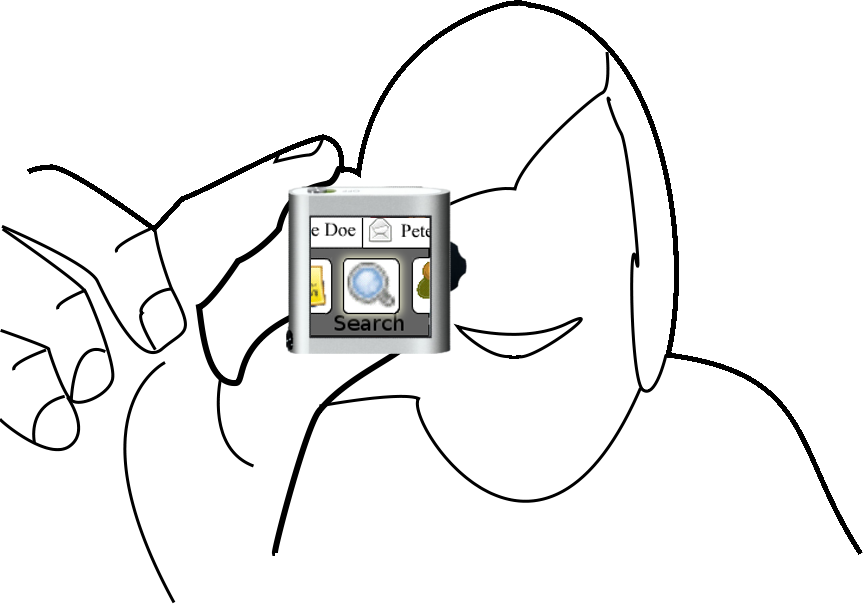
\includegraphics[width=0.8\linewidth]{imgs/main.png}
  \end{center}
  \caption{The SocioPath Device in Context}
  \label{fig:main}
\end{figure}
